\documentclass[a4paper,12pt]{article}
\usepackage[english,ukrainian,russian]{babel}
\linespread{1}
\usepackage{ucs}
\usepackage[utf8]{inputenc}
\usepackage[T2A]{fontenc}
\usepackage[paper=portrait,pagesize]{typearea}
\usepackage{amsmath}
\usepackage{bigints}
\usepackage{amsfonts}
\usepackage{graphicx}
\usepackage{amssymb}
\usepackage{cancel}
\usepackage{gensymb}
\usepackage{multirow}
\usepackage{rotate} 
\usepackage{pdflscape}
\usepackage{bigstrut}
\usepackage[pageanchor]{hyperref}
\usepackage{chngpage}
\usepackage{fancybox,fancyhdr}
\newcommand\tab[1][1cm]{\hspace*{#1}}
\newcommand{\RomanNumeralCaps}[1]{\MakeUppercase{\romannumeral #1}}
\usepackage[left=20mm, top=20mm, right=15mm, bottom=15mm, nofoot]{geometry}


\begin{document}
    \pagestyle{fancy}
    \fancyhead{}
    \fancyhead[R]{ФІ-12 Завалій Олександр}
    \begin{center}
        \large{\textbf{Міністерство освіти і науки України\\
                Національний технічний університет України\\
                «Київський політехнічний інститут імені Ігоря Сікорського»\\
                Навчально-науковий Фізико-технічний інститут}}\\
        \hfill \break \hfill \break \hfill\break \hfill \break \hfill \break \hfill \break \hfill \break
        \hfill \break \hfill \break \hfill \break
        \begin{center}
            \normalsize{\textbf{ОПЕРАЦІЙНІ СИСТЕМИ\\
            Комп’ютерний практикум\\
            Робота №7}}
        \end{center}
    \end{center}
    \hfill \break \hfill \break \hfill \break \hfill \break \hfill \break \hfill \break \hfill \break
    \hfill \break \hfill \break \hfill \break \hfill \break 
    \begin{flushright}
        \large{ \hspace{35pt} Виконав:\\
            студент групи ФI-12\\
            Завалій Олександр\\} 
        \large{ \hspace{35pt} Перевірив:\\
        Кірієнко О.В.} 
    \end{flushright}
    \hfill \break \hfill \break \hfill \break \hfill \break \hfill \break \hfill \break \hfill \break
    \hfill \break
    \begin{center} \textbf{Київ-2023} \end{center}
    \thispagestyle{empty}

\newpage
    \begin{center}
        \section*{\bfseries{Робота №7.\\
        Основи роботи з потоками у Linux з використанням бібліотеки pthread }}
    \end{center}
    \textbf{Мета:} \\
    \hangindent=1.5cm 
    \hangafter=+1 \noindent
    Оволодіння практичними навичками роботи з потоками POSIX у Linux з використанням бібліотеки pthread. \\
    \begin{center}
        \Large{Варіант №5}
    \end{center}
    Зміст індивідуального завдання:
    \begin{enumerate}
        \item \textbf{Створення потоку.} Напишіть програму, що створює потік.
        Застосуйте атрибути за умовчанням. Батьківський і дочірній потоки мають роздрукувати по десять рядків тексту.
        \item \textbf{Очікування потоку.} Модифікуйте програму п. 1 так, щоб
        батьківський потік здійснював роздрукування після завершення дочірнього (функція pthread\_join()).
        \item \textbf{Параметри потоку.} Напишіть програму, що створює чотири потоки, що виконують одну й ту саму функцію.
        Ця функція має роздруковувати послідовність текстових рядків, переданих як параметр. Кожний зі створених
        потоків має роздруковувати різні послідовності рядків.
        \item \textbf{Примусове завершення потоку.} Дочірній потік має роздруковувати текст на екран. Через дві секунди після
        створення дочірнього потоку, батіківський потік має перервати його (функція pthread\_cancel()).
        \item \textbf{Обробка завершення потоку.} Модифікуйте програму п.4 так, щоб дочірній потік перед завершенням
        роздруковував повідомлення про це (pthread\_cleanup\_push()).
    \end{enumerate}

\newpage
    \begin{center}
        \Large{Task \RomanNumeralCaps{1}}
    \end{center}
    \textbf{Створення потоку.} Напишіть програму, що створює потік.
    Застосуйте атрибути за умовчанням. Батьківський і дочірній потоки мають роздрукувати по десять рядків тексту.
    \begin{figure}[h!]
        \begin{minipage}[h]{1\linewidth}
            \centering
            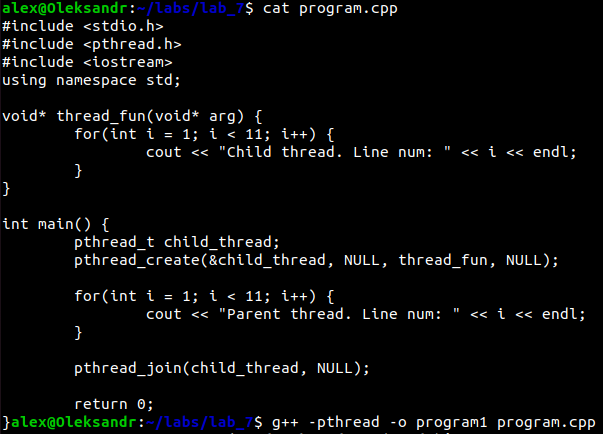
\includegraphics[width=0.6\linewidth]{Prt sc/Figure_1_1.png}  
        \end{minipage}
    \end{figure}
    \begin{figure}[h!]
        \begin{minipage}[h]{1\linewidth}
            \centering
            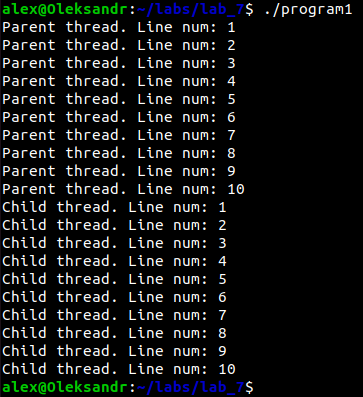
\includegraphics[width=0.5\linewidth]{Prt sc/Figure_1_2.png}  
        \end{minipage}
    \end{figure}

\newpage
    \begin{center}
        \Large{Task \RomanNumeralCaps{2}}
    \end{center}
    \textbf{Очікування потоку.} Модифікуйте програму п. 1 так, щоб
    батьківський потік здійснював роздрукування після завершення дочірнього (функція pthread\_join()).
    \begin{figure}[h!]
        \begin{minipage}[h]{1\linewidth}
            \centering
            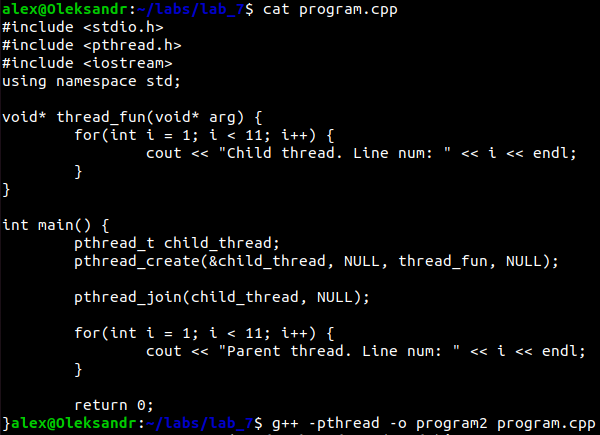
\includegraphics[width=0.6\linewidth]{Prt sc/Figure_2_1.png}  
        \end{minipage}
    \end{figure}
    \begin{figure}[h!]
        \begin{minipage}[h]{1\linewidth}
            \centering
            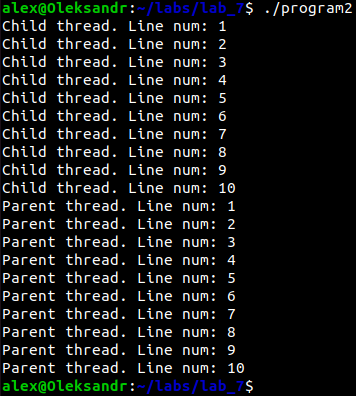
\includegraphics[width=0.6\linewidth]{Prt sc/Figure_2_2.png}  
        \end{minipage}
    \end{figure}

\newpage
    \begin{center}
        \Large{Task \RomanNumeralCaps{3}}
    \end{center}
    \textbf{Параметри потоку.} Напишіть програму, що створює чотири потоки, що виконують одну й ту саму функцію.
    Ця функція має роздруковувати послідовність текстових рядків, переданих як параметр. Кожний зі створених
    потоків має роздруковувати різні послідовності рядків.
    \begin{figure}[h!]
        \begin{minipage}[h]{1\linewidth}
            \centering
            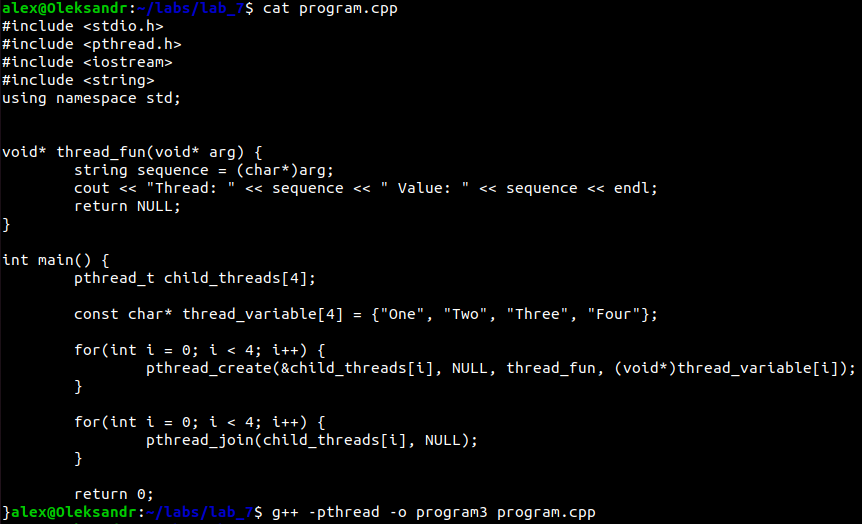
\includegraphics[width=0.6\linewidth]{Prt sc/Figure_3_1.png}  
        \end{minipage}
    \end{figure}
    \begin{figure}[h!]
        \begin{minipage}[h]{1\linewidth}
            \centering
            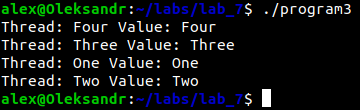
\includegraphics[width=0.6\linewidth]{Prt sc/Figure_3_2.png}  
        \end{minipage}
    \end{figure}
    \begin{center}
        \Large{Task \RomanNumeralCaps{4}}
    \end{center}
    \textbf{Примусове завершення потоку.} Дочірній потік має роздруковувати текст на екран. Через дві секунди після
    створення дочірнього потоку, батіківський потік має перервати його (функція pthread\_cancel()).
    \begin{figure}[h!]
        \begin{minipage}[h]{1\linewidth}
            \centering
            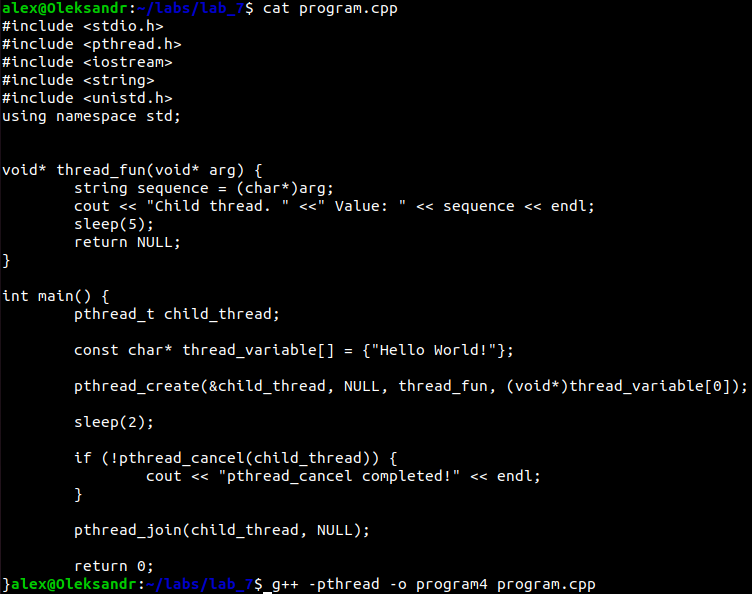
\includegraphics[width=0.6\linewidth]{Prt sc/Figure_4_1.png}  
        \end{minipage}
    \end{figure}

\newpage
    \begin{figure}[h!]
        \begin{minipage}[h]{1\linewidth}
            \centering
            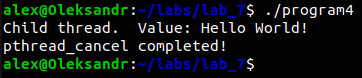
\includegraphics[width=0.6\linewidth]{Prt sc/Figure_4_2.png}  
        \end{minipage}
    \end{figure}
    \begin{center}
        \Large{Task \RomanNumeralCaps{5}}
    \end{center}
    \textbf{Обробка завершення потоку.} Модифікуйте програму п.4 так, щоб дочірній потік перед завершенням
    роздруковував повідомлення про це (pthread\_cleanup\_push()).
    \begin{figure}[h!]
        \begin{minipage}[h]{1\linewidth}
            \centering
            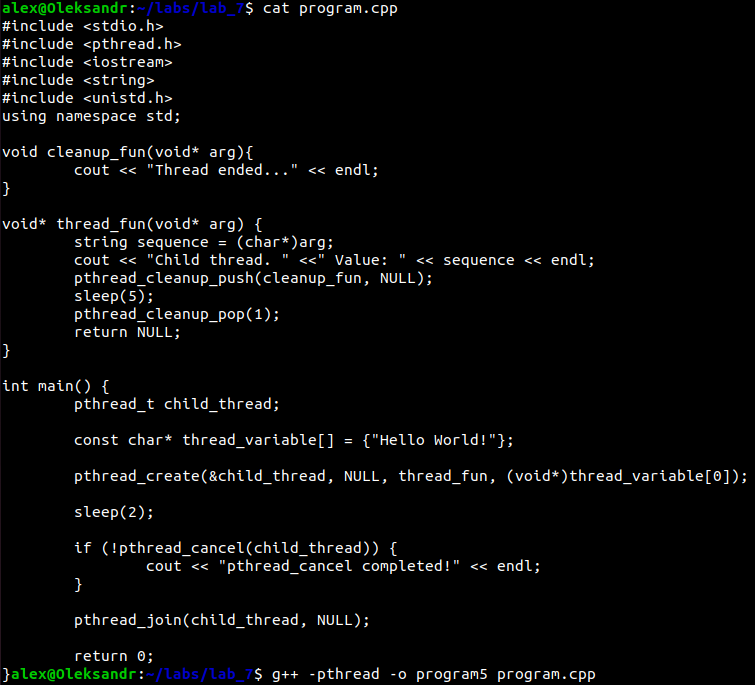
\includegraphics[width=0.6\linewidth]{Prt sc/Figure_5_1.png}  
        \end{minipage}
    \end{figure}
    \begin{figure}[h!]
        \begin{minipage}[h]{1\linewidth}
            \centering
            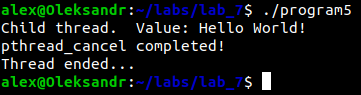
\includegraphics[width=0.6\linewidth]{Prt sc/Figure_5_2.png}  
        \end{minipage}
    \end{figure}

\newpage
    \begin{center}
        \Large{Висновки}
    \end{center}

    Потоки дозволяють розпаралелити виконання програм, що дозволяє ефективніше використовувати ресурси системи.
    POSIX Threads або Pthread — стандарт POSIX реалізації потоків виконання, який визначає API для створення та управління.
    Ця бібліотека може допомогти уникнути гонки даних, блокування та взаємоблокування, тощо.
    Важливо правильно проектувати та розробляти багатопотокові програми.

    Всі процедури Pthreads можуть бути розділені на 4 категорії за призначенням:
    \begin{itemize}
        \item Управляння потоками - створення, об'єднання потоків та інше.
        \item Mutex.
        \item Умовні змінні.
        \item Синхронізація потоків з використанням блокування (lock) і бар'єрів (barriers).
    \end{itemize}

    Використання цих механізмів може допомогти досягти коректної взаємодії між потоками та запобігти виникненню помилок.

    Основні операції з потоками включають створення потоку <<pthread\_create()>>,  завершення потоку <<pthread\_exit()>>, 
    відміна потоку <<pthread\_cancel()>>, блокування потоку до завершення іншого потоку <<pthread\_join()>>, тощо.

    Одним з ключових аспектів роботи з потоками є синхронізація доступу до спільних ресурсів:
    \begin{itemize}
        \item pthread\_mutex\_init (), pthread\_mutex\_destroy (), pthread\_mutex\_lock (), \\
        pthread\_mutex\_trylock (), pthread\_mutex\_unlock (): за допомогою mutex.
        \item pthread\_cond\_init(), pthread\_cond\_signal, pthread\_cond\_wait(): за допомогою умовних змінних.
    \end{itemize}

    Залишаються типи даних при роботі з потоками. Всього існує лише два типи:
    \begin{itemize}
        \item pthread\_t: дескриптор потоку.
        \item pthread\_attr\_t: набір атрибутів потоку.
    \end{itemize}

\end{document}